\section{Case}

\subsection{Description of the case}

\paragraph{}The aim of this project is to analyze the airflow inside the first stages of a turbofan. The turbofan consists of an initial stage where a fan is placed. This first stage increases the pressure of the air that goes through it and, as it can be seen in \ref{turbofanparts}, a part of the incoming airflow goes to the low pressure compression stage (main or primary flow) and the other goes to the conducts (secondary flow). As the secondary flow advances through the conduct, the main flow enters the engine core where it goes through the low pressure and high pressure compression stages. By increasing the pressure of the air, the density also increases; thus, a higher mass flow can be mixed with the fuel and burned in the combustion chamber. After this process, the gases go through the turbines, interchanging energy with them (pressure and velocity, mainly), and they arrive at the nozzle, where the air is accelerated, and a thrust force is obtained.

\begin{figure}[h!]
\centering
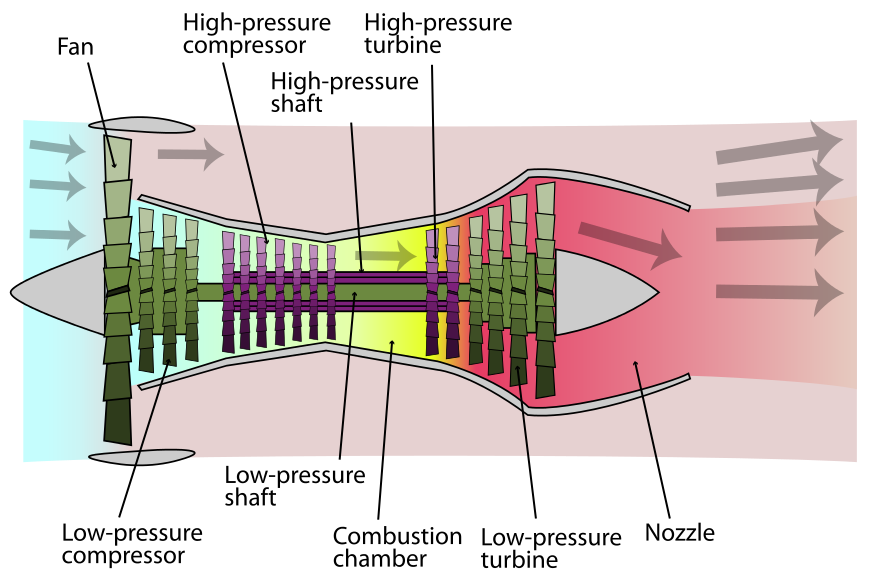
\includegraphics[scale=0.45]{./img/TurbofanEtapas.png}
\caption{Parts of a turbofan}
\label{turbofanparts}
\end{figure}

\paragraph{}To simulate the flow in the first stages of the turbofan, we have downloaded the following turbine model from \textit{GrabCad}, shown in \ref{turbinegrabcad}. This model is pretty similar with the one shown above (\ref{turbofanparts}) and the simulation will take place between the back side of the fan and the back side of the second compressor.

\paragraph{}The geometry of the \textit{blockMesh} as well as the refined mesh of this parts will be shown and discussed in the next section.


\begin{figure}[h!]
\centering
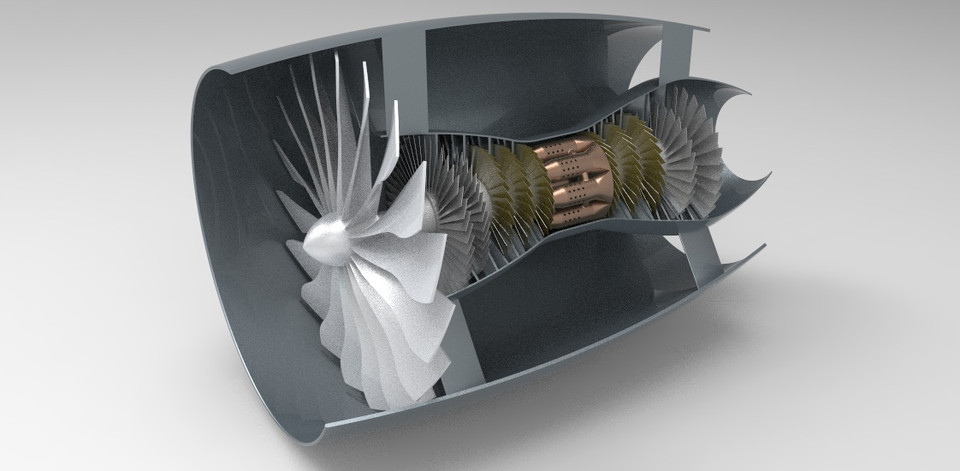
\includegraphics[scale=0.54]{./img/Turbofan.png}
\caption{Model used}
\label{turbinegrabcad}
\end{figure}

\subsection{Hypotheses}

\paragraph{}Given that we are not able to use a supercomputer and the computational power that is available to us is very limited (since we are using our own personal computers to run this simulation), several hypotheses have to be made to alleviate the calculation time. These hypotheses are presented below.

\begin{itemize}
	\item Viscous flow
	\item Incompressible flow
	\item Newtonian flow
	\item Stationary flow
\end{itemize}

\paragraph{}Clearly, the flow is not incompressible; the aim of the turbofan is to compress the air to pursue a more efficient combustion. However, the compressible solvers are really difficult to use and the computation time is also higher given that we have a high number of control volumes (as discussed in the next section). \\
So, the simulation will take into account that it is a tridimensional, that it behaves as a newtonian fluid and it will be run under stationary flow conditions (that is: the velocity in the inlet is always uniform and has a fixed value).